\section{Lattices and continuation of schedules}
\label{sec:lattice-continuation}

A real basis of roots need not be an integral basis of the root lattice.
Thus the endpoint balance of the basic schedule does not by itself make
its switch coefficients integral.  We identify the type-$D$ obstruction
and construct a deformation that removes it when a suitable local
modification is available.  Section~\ref{sec:moment-knots} will force
such a modification.

The result concerns the switch condition in Definition~\ref{def:schedule},
not the stronger chain condition in a highest-weight path model.  An
integral chain in the Lakshmibai--Seshadri model for a dominant weight
$\theta$ must be saturated in the Bruhat order on $W/W_\theta$
\cite[Section~2.2]{Lit94}; the distinction also appears in
\cite[Theorem~5.6]{KM08}. The passage from integral switches to
representations remains separate.

\begin{theorem}[Integral schedules]\label{thm:integral-schedule}
Let the three labels have integral root pairings and satisfy
\(\lambda+\mu-\xi\in Q\), and let \(\eta\) be any polygonal shape with
dominant increments and endpoint \(\mu\).  A real moment solution gives an
integral schedule in either of the following cases:
\begin{enumerate}[label=\textup{(\roman*)}]
\item the root system is a permutation system;
\item the root system is \(D_l\), and \(\mu\) has at most one zero
coordinate.
\end{enumerate}
An orthogonal central space is allowed in either case; its equation is
ordinary vector addition.
\end{theorem}

For a permutation system, a root basis is a spanning tree in each
semisimple factor and is an integral basis of its root lattice.
Proposition~\ref{prop:basic-schedule} and the endpoint balance therefore
prove the first assertion.  We prove the second by induction on \(l\).
Throughout this section, uses of Theorem~\ref{thm:integral-schedule} in
orthogonal blocks refer only to strictly smaller ranks.

\subsection{Blocks, parity, and the exceptional graph}

Associate a signed graph on the coordinate axes to a collection of
\(D_l\)-roots.  An edge \(e_i-\varepsilon e_j\), with
\(\varepsilon\in\{1,-1\}\), imposes the signed identification
\(x_i=\varepsilon x_j\).  A connected component is \emph{balanced} if
these identifications are consistent around every cycle.  Changing the
signs of its axes then makes its roots a permutation system.  An
unbalanced component has full coordinate span.
This is the signed-graphic representation of the classical root
systems studied by Zaslavsky \cite{Zas82,Zas12}. We will also need its
integer-lattice information, which is proved below by leaf removal
and the cycle equations.

\begin{lemma}[Combining blocks]\label{lem:block-reduction}
Suppose a moment solution splits into commuting coordinate blocks of
permutation type and orthogonal type.  Assign the initial, moving, and
final coordinates using this splitting.  Under the hypotheses of
Theorem~\ref{thm:integral-schedule}\textup{(ii)}, integral schedules can be
combined from the blocks.  In particular, induction applies if there is
a permutation block, if there are at least three proper orthogonal
blocks, or if there are two proper orthogonal blocks of even parity.
Here the parity of an orthogonal block is the sum, modulo two, of its
assigned difference \(\lambda+\mu-\xi\).
\end{lemma}

\begin{proof}
We first explain the assignments and their arithmetic.  In a schedule
whose roots lie in the stated blocks, the initial moving frame assigns
shape coordinates to each block; the endpoint assigns the final
coordinates.  Restricting the schedule gives a moment solution in the
block by Lemma~\ref{lem:schedule-moment}.  Conversely, after sorting the
assigned moving weight for the block, all restricted shape increments
are dominant in the same frame.  Indeed every root comparison has the
same weak sign on every dominant increment as on their sum.  The
orthogonal central coordinates are simply retained.  Schedules obtained
in the blocks can thus be superposed.  Their root inequalities are
internal to the blocks, so no comparison with an outside coordinate is
required.

The same assignments are available for a matrix splitting.  Choose an
oriented adapted orthonormal frame, and then choose representatives of
each of the three matrices in its blocks.  The assembled representatives
belong to the original special-orthogonal orbits.  For the negative end
matrix, negate its representative to obtain the assigned end label for
addition.  Subgroup Weyl actions on these assignments are permitted in
the full Weyl coset; a different initial representative can finally be
returned to \(\lambda\) by a common Weyl action on the path.

Each type-\(D\) weight has a uniform coordinate fractional part, zero or
one-half, invariant under signed permutations.  The global root-lattice
condition consequently makes every assigned coordinate difference an
integer.  On a permutation block, the central equation gives zero
signed sum.  Its difference lies in the permutation root lattice and
has even ordinary sum as well.  On an orthogonal block, changing allowed
representatives changes the difference by a block root, so its parity
is well-defined.  The number of odd orthogonal blocks is even.

Even orthogonal blocks can be solved separately by induction; odd ones
can be joined in pairs, using their direct-sum moment solution in the
larger orthogonal block.  If there are at least three orthogonal blocks,
every such union is still proper.  If there is a permutation block, all
orthogonal blocks together occupy a proper subspace and have even total
parity; solve that union and the permutation blocks separately.  A
single permutation block on all axes is covered by the first assertion
of the theorem.  A real two-dimensional orthogonal block has only its
central equation and is even.  Finally, a restriction of the moving
coordinates retains the at-most-one-zero hypothesis.
\end{proof}

One useful source of a permutation block is a nonzero common commuting
real skew-symmetric operator.  Its kernel is an orthogonal block.  On
each subspace belonging to a nonzero absolute eigenvalue, its normalized
restriction is a complex structure; the commuting skew matrices become
Hermitian matrices and give a permutation-type addition problem.  Thus
Lemma~\ref{lem:block-reduction} applies to this splitting, also inside an
already assigned orthogonal block.

\begin{lemma}[The exceptional case]\label{lem:hard-case}
If no integral schedule exists, any real schedule with at most \(l\)
switches has exactly \(l\) independent switch roots, and its graph has
exactly two connected components, both unbalanced and of odd parity.
Each component is unicyclic.  On its cycle the switch coefficients are
half-odd-integers, and off the cycle they are integers.
\end{lemma}

\begin{proof}
If the roots have deficient span, some connected component is balanced,
possibly an isolated axis.  Lemma~\ref{lem:block-reduction} applies.
Otherwise there are exactly \(l\) independent roots.  Each component is
then unbalanced and has as many edges as vertices, hence has a single
cycle.

The roots of an unbalanced unicyclic component generate precisely its
even-sum integer lattice.  To see this, remove leaves successively.
Their coefficients are determined integrally by the corresponding
coordinate equations.  The remaining cycle equations determine all
cycle coefficients from one of them, with integral differences or
sums; inconsistency of the signs closes the final equation with a
factor two.  The resulting determinant has absolute value two, so the
image is the even-sum lattice.  The coefficients are integral when the
right-hand side has even coordinate sum and all half-odd-integral on
the cycle when its coordinate sum is odd.  This argument includes an
unbalanced cycle with two edges.

A connected graph therefore already gives integral switch levels.
Multiple components can be treated by
Lemma~\ref{lem:block-reduction}, except for exactly two odd orthogonal
components.  These are the only possibility under the assumed failure
of integral realizability.
\end{proof}

In particular the induction starts in every rank too small to contain
two unbalanced components.  Notice also that the reduction applies to
any real schedule with at most \(l\) switches, not just to the original
basis schedule.  For example, a connected balanced graph with \(l\)
edges gives a permutation reduction, although it is not a root basis.

\begin{lemma}[Closedness and generic shapes]\label{int:closedness}
For fixed labels, the existence of an integral schedule is closed under
uniform convergence of shapes with dominant increments.  It suffices
to prove Theorem~\ref{thm:integral-schedule} for polygonal shapes whose
slopes are relatively interior to the smallest chamber face containing
\(\mu\), with generic break values in that face.
\end{lemma}

\begin{proof}
Delete zero-total, endpoint-time, and zero-gap switches by the
simplifications in Definition~\ref{def:schedule}.  These operations
preserve integrality.  For the remaining strict switches, a small
regular perturbation and chamber projection gives a strictly downward
Bruhat step at each switch.  Their number is therefore at most the
length of the longest Weyl element.  This bound is independent of the
shape.  There are finitely many ordered root lists and initial frames;
after taking a subsequence they are constant and their times converge.
The switch levels are bounded integers, hence are also constant on a
further subsequence.  Passing to the limit preserves the endpoint,
weak signs, and these integer levels.

Let \(F\) be the smallest chamber face containing \(\mu\).  Every
increment of every allowed shape lies in \(F\): a simple-root pairing
which vanishes on \(\mu\) is a sum of nonnegative increment pairings,
each of which must vanish.  Slight interpolation with the straight
shape \(t\mu\) makes all slopes relatively interior to \(F\).
Subdivision and perturbation of break values, keeping the endpoint,
then impose any finite collection of open dense genericity conditions.
The precise conditions used below are given in
Section~\ref{sec:moment-knots}.
\end{proof}

We may now assume that there is no integral schedule for such a shape.
Take the schedule from Proposition~\ref{prop:basic-schedule}.
Lemma~\ref{lem:hard-case} gives two odd components, denoted \(P,Q\).
Every switch has positive gap and positive total and lies at an interior
time: deleting a zero sign or a boundary switch would leave at most
\(l-1\) switches.  Retain also the limiting cover property of this
particular schedule.  It will be used only in the counting argument,
not as a condition on its later deformations.

\subsection{The half-relation deformation}

We seek to replace a cluster of the exceptional schedule by a cluster
with one additional switch.  Outside that cluster the modification
must be recoverable by undoing a suffix reflection or a change of
moving frame that fixes the shape.  First consider the lattice part
of this problem: an exact local modification with \(k=l+1\) ordered
roots generating \(Q(D_l)\).  Such a list need not retain all the old
roots.  We will move its coefficients to integers without changing
its endpoint; the local-link conditions below will supply the
feasibility needed to begin that motion.  Write
\[
 p_i=s_{\beta_i}\cdots s_{\beta_1},\qquad p_0=1,
 \qquad \gamma_i=p_{i-1}^{-1}\beta_i,
 \qquad b=w_{\mathrm{in}}\eta.
\]
Thus \(\gamma_i\) is the switch root in the initial velocity frame, and
\(m_i=-\gamma_i\cdot b(t_i)\).  The two endpoint balances are
\begin{align}
 y(1)&=\lambda+p_k b(1)-\sum_{i=1}^k m_i\beta_i,
 \label{int:position-balance}\\
 p_k^{-1}y(1)&=\lambda+b(1)-\sum_{i=1}^k G_i\gamma_i,
 \label{int:velocity-balance}
\end{align}
where
\begin{equation}\label{int:gap}
 G_i=\lambda\cdot\beta_i
       -\sum_{j<i}m_j\,\beta_j\cdot\beta_i-m_i.
\end{equation}
The first identity is the schedule balance; the second follows by
reflecting the position back at every switch.  Formula~\eqref{int:gap}
also shows that the change from \(m\) to \(G\) is affine integral and
unimodular, with diagonal coefficients \(-1\).

\begin{lemma}[Half-kernel bounds and potential]\label{int:half-kernel}
Suppose the \(l+1\) roots generate \(Q(D_l)\), and their exact base
coefficients \(m^0\) are half-integral.  If \(m^0\) is not already
integral, either orientation \(d\) of half the primitive integer
relation among the roots satisfies
\begin{equation}\label{int:half-bounds}
 m^0+d\in\Z^{l+1},\qquad |d_i|\le1,\qquad |d_i^G|\le1,
\end{equation}
where \(d^G\) is its image under the linear part of
\eqref{int:gap}.  Moreover, there is a vector \(L\) such that
\begin{equation}\label{int:potential-direction}
 d_i=L\cdot\gamma_i\quad(1\le i\le l+1).
\end{equation}
\end{lemma}

\begin{proof}
A full-rank signed graph with \(c\) unbalanced components generates an
integer lattice of index \(2^c\).  Thus a graph generating \(Q(D_l)\)
is connected and unbalanced.  Deleting one edge leaves at most two
components.  Each nonzero maximal minor consequently has absolute
value two or four: its components are unbalanced unicyclic graphs.
Their gcd is two, the index of \(Q(D_l)\) in \(\Z^l\).  Cofactors
therefore give a primitive kernel vector with entries of magnitude at
most two.

The velocity roots generate the same lattice as the position roots:
\(\gamma_i\) equals \(\beta_i\) plus an integral combination of earlier
roots, with a triangular inverse of the same form.  Applying the
preceding minor argument in that frame, and using the unimodular
coefficient change \eqref{int:gap}, proves both derivative bounds.
The endpoint right-hand side in \eqref{int:position-balance} lies in
\(Q(D_l)\), so it has an integer coefficient vector.  Its difference
from \(m^0\) is a multiple of the primitive relation.  Since that
relation has relatively prime entries and \(m^0\) is half-integral but
not integral, the multiple is half-odd-integral.  Adding either half
relation makes all coefficients integral.

Finally, telescoping the reflections gives
\begin{equation}\label{int:telescoping}
 \sum_i (L\cdot\gamma_i)\beta_i=(1-p_k)L.
\end{equation}
The determinant of \(p_k\) is \((-1)^{l+1}\).  An orthogonal operator
in dimension \(l\) without eigenvalue \(+1\) has determinant
\((-1)^l\), by pairing its nonreal eigenvalues.  Hence \(p_k\) has a
nonzero fixed vector.  Since the \(\gamma_i\) span, its pairings with
them give a nonzero relation.  The relation space is one-dimensional;
scaling this fixed vector proves \eqref{int:potential-direction}.
\end{proof}

We vary the coefficients by
\begin{equation}\label{int:interpolation}
 m(s)=m^0+s d,\qquad 0\le s\le1.
\end{equation}
At parameter one every coefficient is integral, and the position
balance keeps the endpoint fixed.  This line of coefficient vectors
is not yet a family of schedules.  The time for its \(i\)-th switch
must solve
\[
 -\gamma_i\cdot b(t_i(s))=m_i(s).
\]
A positive total makes the left side strictly increasing along our
relatively regular shape, so it has a local inverse at an interior
base time.  These inverse times are candidates: they need not occur
in the prescribed order, and their position gaps must remain
nonnegative.  We must start the motion at the modified cluster and
then continue it through collisions without losing these conditions.

Here is the exact form of the local input we shall use.  A
\emph{local link} modifies the original schedule at one time, replacing
some of its switches by one more switch in total, such that:
\begin{enumerate}[label=\textup{(\alph*)}]
\item the new \(l+1\) roots generate \(Q(D_l)\), and the exact base
coefficients are half-integral;
\item one orientation of \(d\) in \eqref{int:interpolation} gives
admissible, weakly ordered candidate switches within the modified
cluster for all sufficiently small positive \(s\), allowing
commutations of disjoint switches;
\item at the other time clusters the modification can be forgotten,
either by a common reflection of the suffix or by a discrepancy of
moving frames that fixes the entire shape.
\end{enumerate}
In the latter alternative, equality of assigned moving weights is
sufficient.  Indeed \(W_\mu\) fixes the face \(F\) in
Lemma~\ref{int:closedness} pointwise.  If
\(w'\mu=w\mu\), then \(w^{-1}w'\in W_\mu\), and therefore
\begin{equation}\label{int:whole-shape}
 w'\eta(t)=w\eta(t)\qquad\text{for every }t.
\end{equation}
Thus a local reassignment of equal moving values preserves every later
shape value, not just the value at the modified time.

Figure~\ref{fig:half-relation} shows the lattice calculation in the
simplest joining-root case.  Its half-relation reaches integer
coefficients; the local-link conditions are what permit those
coefficients to be realized by nearby switch times.
\begin{figure}[tb]
\centering
\begin{tikzpicture}[
  x=1cm,y=1cm,
  axis/.style={circle,draw,fill=white,inner sep=1.6pt},
  root/.style={line width=.7pt},
  newroot/.style={line width=1.2pt,blue!60!black},
  every node/.style={font=\small}]
  \node[axis] (p0) at (0,0) {};
  \node[axis] (p1) at (1.3,.85) {};
  \node[axis] (p2) at (1.3,-.85) {};
  \node[axis] (q0) at (4.3,0) {};
  \node[axis] (q1) at (5.6,.85) {};
  \node[axis] (q2) at (5.6,-.85) {};
  \draw[root] (p0)--(p1)--(p2);
  \draw[root,dashed] (p2)--(p0);
  \draw[root] (q0)--(q1)--(q2);
  \draw[root,dashed] (q2)--(q0);
  \draw[newroot] (p1)--node[above,sloped] {new joining root}
    node[below,sloped] {$|d_e|=1$} (q0);
  \node at (.65,1.45) {$P$: odd assigned parity};
  \node at (4.95,1.45) {$Q$: odd assigned parity};
  \node[align=center] at (.65,-1.5)
    {cycle: $m_e^0\in\Z+\tfrac12$\\$|d_e|=\tfrac12$};
  \node[align=center] at (4.95,-1.5)
    {cycle: $m_e^0\in\Z+\tfrac12$\\$|d_e|=\tfrac12$};
  \draw[root] (0,-2.3)--(.5,-2.3);
  \node[anchor=west] at (.6,-2.3) {equal-sign identification};
  \draw[root,dashed] (0,-2.8)--(.5,-2.8);
  \node[anchor=west] at (.6,-2.8) {opposite-sign identification};
\end{tikzpicture}
\caption{The graph underlying the half-relation deformation.
The two original components are unbalanced and have odd assigned
difference parity. A joining root connects their even-sum lattices
inside the full type-$D$ root lattice. For the displayed graph,
half the primitive relation has absolute value $\tfrac12$ on the
cycles and $1$ on the joining edge. More generally the latter
value occurs on the whole connecting path, and coefficients on
other attached trees vanish. Cycle lengths and omitted branches
are schematic; local feasibility is supplied by a local link.}
\label{fig:half-relation}
\end{figure}


\subsection{Sorting collisions and continuing a link}

\begin{proposition}[Continuation]\label{prop:continuation}
Under the standing assumption of no integral schedule, a local link
cannot exist.
\end{proposition}

\begin{proof}
Continuation may replace the ordered root list when times collide.
We therefore follow coefficient lines in a finite set of root lists,
not one fixed list.  Each replacement preserves the endpoint and
transforms the extrapolated coefficients at parameter one by an
integral unimodular change.  First we exclude removable switches at
an interior parameter.  We then use a common potential to select
compatible times for alternative routes through a tied cluster.
The local-link conditions start the motion at parameter zero, and
compactness carries it to parameter one.

\paragraph{Strictness at a continuation point.}
Suppose an exact augmented schedule occurs at a parameter
\(0<s_*<1\), with a primitive half-kernel direction and integral
extrapolation at one.  If a switch is at time zero or one, its
coefficient is integral; a zero-total switch has coefficient zero.
Consequently
\[
 (1-s_*)d_i=m_i(1)-m_i(s_*)\in\Z,
 \qquad |(1-s_*)d_i|<1,
\]
so \(d_i=0\).  Deleting that switch leaves a nonzero relation among
at most \(l\) roots, hence deficient rank.  At an endpoint one may
delete the entire endpoint cluster.  Either operation contradicts
Lemma~\ref{lem:hard-case}.

If a gap is zero, the same reasoning applied to \(G_i\) gives
\(d_i^G=0\), since the extrapolated gap is integral by
\eqref{int:gap}.  Reflect the suffix and delete the switch.  All
remaining velocity roots are unchanged: reflection changes both their
position labels and the accumulated frame by the same factor, which
cancels in \(p_{i-1}^{-1}\beta_i\).  The residual dependence again gives
deficient rank.  Thus all switches at such a parameter are interior,
with strict gaps and totals.

At \(s_*=0\) this arithmetic would not exclude a nonzero half-kernel
entry.  Instead, in an \emph{unaffected} cluster use the forgetting
property of the local link.  Any reordering there preserving its full
reflection product and exact displacement can also be performed after
forgetting the augmentation.  In case \eqref{int:whole-shape}, the same
fixed right stabilizer discrepancy persists after the reordering; in
the reflected-suffix case conjugate the reordered roots back.
One obtains an exact schedule with the original \(l\) switches.
A zero sign or boundary switch could then be removed, leaving at most
\(l-1\) switches, again impossible.  This argument applies after every
successive reordering at that base time.

\paragraph{A common potential at a collision.}
Suppose several candidate times coincide at \(\tau\) when \(s=s_*\).
By Lemma~\ref{int:half-kernel}, throughout that cluster
\begin{equation}\label{int:cluster-potential}
 m_i(s)=\gamma_i\cdot\bigl(-b(\tau)+(s-s_*)L\bigr).
\end{equation}
The candidate time belonging to a root line \(\gamma\) therefore solves
\begin{equation}\label{int:candidate-time}
 \gamma\cdot\bigl(b(t)-b(\tau)+(s-s_*)L\bigr)=0.
\end{equation}
It depends only on that root line and the common potential, not on the
route chosen through the cluster.

Commute an adjacent pair with orthogonal roots whenever its candidate
times are inverted.  For a nonorthogonal pair, the rank-two subsystem
is \(A_2\).  At the base point choose one regular refinement of the
common position order and one of the incoming velocity order,
preserving their strict inequalities, and transport the latter
through the two reflections.  The two steps are decreasing in this
single rank-two Bruhat order.  Both are covers: their length drops
are positive odd integers whose sum is at most three, hence their
sum is two.  Every length-two interval in the \(A_2\) Bruhat order is
a diamond.  Its other route therefore also consists of two downward
covers: the position root is positive, and its inverse image under
the current velocity state is negative, at each step.  Forgetting
the common regular refinements gives weakly correct position and
velocity signs for this other route.
Identical consecutive reflection lines cannot occur, since the first
would reverse the strict velocity inequality required by the second.
Replace the pair by that route with the same product.  The preceding
deletion arguments exclude equality before we require its nearby
inverse times.

The displacement of the pair is unchanged by
\eqref{int:cluster-potential} and the telescoping identity
\eqref{int:telescoping}.  Any two nonparallel roots in this \(A_2\)
subsystem form a basis of its root lattice.  Thus the old and new
coefficient pairs are related by an integral unimodular map.  Outside
the pair the accumulated frame, roots, and coefficients are unchanged.
It follows that the full lattice, the primitive half-kernel direction,
and integral extrapolation at one are all preserved.

\paragraph{Termination of sorting.}
Let \(i,j\) denote the simple root lines of the velocity-positive
system and \(h=i+j\) its remaining root line.  Their candidate times
are \(T_i,T_j,T_h\).  Choose representatives consistently with the
incoming moving order, so that their level functions have the same
strict monotonicity.  Reversing a representative does not change its
candidate-time equation.  The left-hand side of
\eqref{int:candidate-time} for \(h\) is the sum of those for \(i,j\);
strict monotonicity implies that \(T_h\) lies strictly between
\(T_i,T_j\) when they differ.  This holds also across a shape break.
The four possible diamonds, written as successive right reflection
labels in the velocity frame, are
\[
\begin{array}{cc}
\toprule
\text{lengths}&\text{alternative routes}\\ \midrule
3\longrightarrow1&ij\ \longleftrightarrow\ jh\\
3\longrightarrow1&ih\ \longleftrightarrow\ ji\\
2\longrightarrow0&ji\ \longleftrightarrow\ hj\\
2\longrightarrow0&ij\ \longleftrightarrow\ hi.\\
\bottomrule
\end{array}
\]
Indeed, writing \(s_h=s_i s_j s_i=s_j s_i s_j\), their products are
\(s_i s_j=s_j s_h=s_h s_i\) and
\(s_j s_i=s_i s_h=s_h s_j\); the starting length determines which
two factorizations form the interval.  These are the same common
position and velocity refinements used above.
In each row, if the current route is descending in candidate time, the
other route has strictly earlier first time.  For example, in the
first row \(T_i>T_j\) makes the route \(jh\) start earlier; conversely
\(T_j>T_h\) implies \(T_j>T_h>T_i\), so \(ij\) starts earlier.
The other three rows follow by the same between-time inequality.
Orthogonal commutation also strictly decreases the first time of the
inverted pair.

The full candidate-time list therefore decreases lexicographically.
Only finitely many root lists are possible, and each root line has its
fixed candidate time from \eqref{int:candidate-time}.  Sorting
terminates in a weakly ordered list.  All its strict gaps and totals
persist in a common sufficiently small neighborhood of the base
parameter, since there are only finitely many possible lists.
At \(s_*=0\) apply this procedure only to unaffected clusters; the
modified cluster is feasible by the definition of a local link.
Consequently the link gives a genuine schedule for small positive
\(s\).

\paragraph{Arrival at the integral endpoint.}
Consider all parameters in \((0,1]\) admitting an augmented schedule
with \(l+1\) lattice-generating roots, a primitive half-kernel
direction, and integral extrapolation at one.  This set is nonempty by
the preceding paragraph.  Root lists, initial frames, and endpoint
representatives range over finite sets.  The actual coefficients are
bounded by the compact shape, and every direction coordinate has
absolute value at most one.  Their extrapolated integer values at one
are therefore bounded as well and range over a finite set.  The
half-kernel directions themselves also range over a finite set.

At the supremum, choose a subsequence fixing all this discrete data.
The ordered switch times have a convergent subsequence; endpoint
balance and weak signs are closed conditions.  Thus the supremum is
feasible.  If it is less than one, the strictness argument excludes
all boundary or removable switches there, and the common-potential
sorting extends feasibility to its right.  This is impossible.
Parameter one is attained, and every coefficient is then integral,
contrary to the standing assumption.
\end{proof}

The proof only asks for weak order inside a feasible modified cluster.
If two new transfers have the same strictly increasing level function
and equal coefficient derivatives, their times remain exactly equal;
the specified order of simultaneous switches is permitted.

\begin{lemma}[Direct links]\label{lem:direct-links}
In the exceptional schedule with components \(P,Q\), each of the
following produces a forbidden local link:
\begin{enumerate}[label=\textup{(\roman*)}]
\item a signed cross-component pair with strict concordant position
and moving-value orders at time zero;
\item a signed cross-component pair with strict discordant orders at
time one;
\item a position crossing of a cross-component pair with distinct
moving values between old switch times;
\item the crossing in \textup{(iii)} at an old switch time, if both
axes are unused by its cluster.
\end{enumerate}
\end{lemma}

\begin{proof}
In the first case insert the cross swap at time zero, choosing the
initial frame so that the old frame occurs just after the swap.
Before the swap the velocity order is the strict inverse of its
position order, so the gap is positive.  Its coefficient is zero.
The position graph has gained a bridge joining the two odd unbalanced
components; its roots generate the full root lattice.  In the
primitive relation the bridge coefficient has magnitude two.  Indeed,
prune the off-cycle branches and follow the remaining connecting path:
the cycle equations give equal coefficient magnitudes around each odd
cycle, and their sign inconsistency makes the connecting flux twice
that magnitude.  Thus the primitive magnitudes are one on the cycles
and two along the connecting path.  The half-kernel derivative on the
bridge has magnitude one.  Choose its sign to
make the new time move into \((0,1)\).  All old gaps remain positive.
The inserted edge can plainly be forgotten at the exact base time.
The end case is the same construction with the old state before the
new swap; choose the derivative to move its time leftward from one.
Its base coefficient is the integral total root pairing.

For a crossing, insert the swap with its strict approaching inversion
and reflect the entire old suffix.  At the base point its gap is zero,
its total is positive, and continuity holds because the crossing
position is fixed by the reflection.  In the velocity frame all old
roots are retained.  The two component root bases in that frame still
generate their respective even-sum lattices, and the new root is a
bridge between them.  Hence the augmented roots generate \(Q(D_l)\),
and the primitive half-kernel direction in the gap coordinates has
nonzero, indeed unit, coordinate on the bridge.  Choose its sign so
that the new gap becomes positive.  Its time remains interior.
Formula~\eqref{int:gap}, with zero base gap, shows that the inserted
coefficient is half-integral; the other base coefficients remain
half-integral.  Forgetting is precisely reflection of the suffix back.

If the crossing lies at an old cluster unused by its two axes, its new
root is orthogonal to all roots in that cluster.  Commute these
switches to put their nearby candidate times in order.  This proves
local feasibility also in the last case.  Proposition~\ref{prop:continuation}
excludes each construction.
\end{proof}

It remains to show that the exceptional schedule necessarily admits a
link.  Proposition~\ref{prop:strict-count} supplies a strict excess of
cross-component comparisons, while Proposition~\ref{prop:knot-count}
shows that this excess cannot disappear without a locally feasible
link.  These two assertions, proved next, complete
Theorem~\ref{thm:integral-schedule}.
